\chapter{From raw specification to fully proven spec: A full example}
\label{ch:fullexample}
%Chapter 9

In this chapter we take a system specification through all the steps of
\gls{zmath} to demonstrate how we can get from a raw specification to a full
proof. We have added commentary throughout so the reader can understand how we
can get from one step to another. We have added figures and screenshots of each
step of the \gls{zmath} framework.

\section{Step 0\\Raw Specification}
We take a raw specification ModuleReg \cite{essenceofz}, which displays students
taking modules in a school environment (shown in figure \ref{fig:rawschema}) The
output for the specification can be seen in figure \ref{fig:rawschemaout}. The
full proof for the ModuleReg specification can be found in \ref{app:moduleregfullproof}.

\begin{figure}[H]
\vspace{-0.2in}
\centering
\begin{minipage}{0.45\textwidth}
\centering
\begin{tiny}
\begin{BVerbatim}
\documentclass{article}
\usepackage{zmathlang}
\begin{document}

\begin{zed}
[PERSON, MODULE]
\end{zed}

\begin{schema}{ModuleReg}
students: \power PERSON \\
degModules: \power MODULE \\
taking: PERSON \rel MODULE
\where
\dom taking \subseteq students \\
\ran taking \subseteq degModules
\end{schema}

\begin{schema}{AddStudent}
\Delta ModuleReg \\
p?: PERSON \\
\where
p? \notin students \\
students' = students \cup \{p?\} \\
degModules' = degModules \\
taking' = taking
\end{schema}

\begin{schema}{RegForModule}
\Delta ModuleReg \\
p?: PERSON \\
m?: MODULE
\where
p? \in students \\
m? \in degModules \\
p? \mapsto m? \notin taking \\
taking' = taking \cup \{p? \mapsto m?\} \\
students' = students \\
degModules' = degModules
\end{schema}
\end{document}
\end{BVerbatim}
\end{tiny}
%\vspace{-0.2in}
\caption{Part of the raw schema.\label{fig:rawschema}}
%\vspace{-0.2in}
\end{minipage}\hfill
\begin{minipage}{0.45\textwidth}
\centering
%\fbox{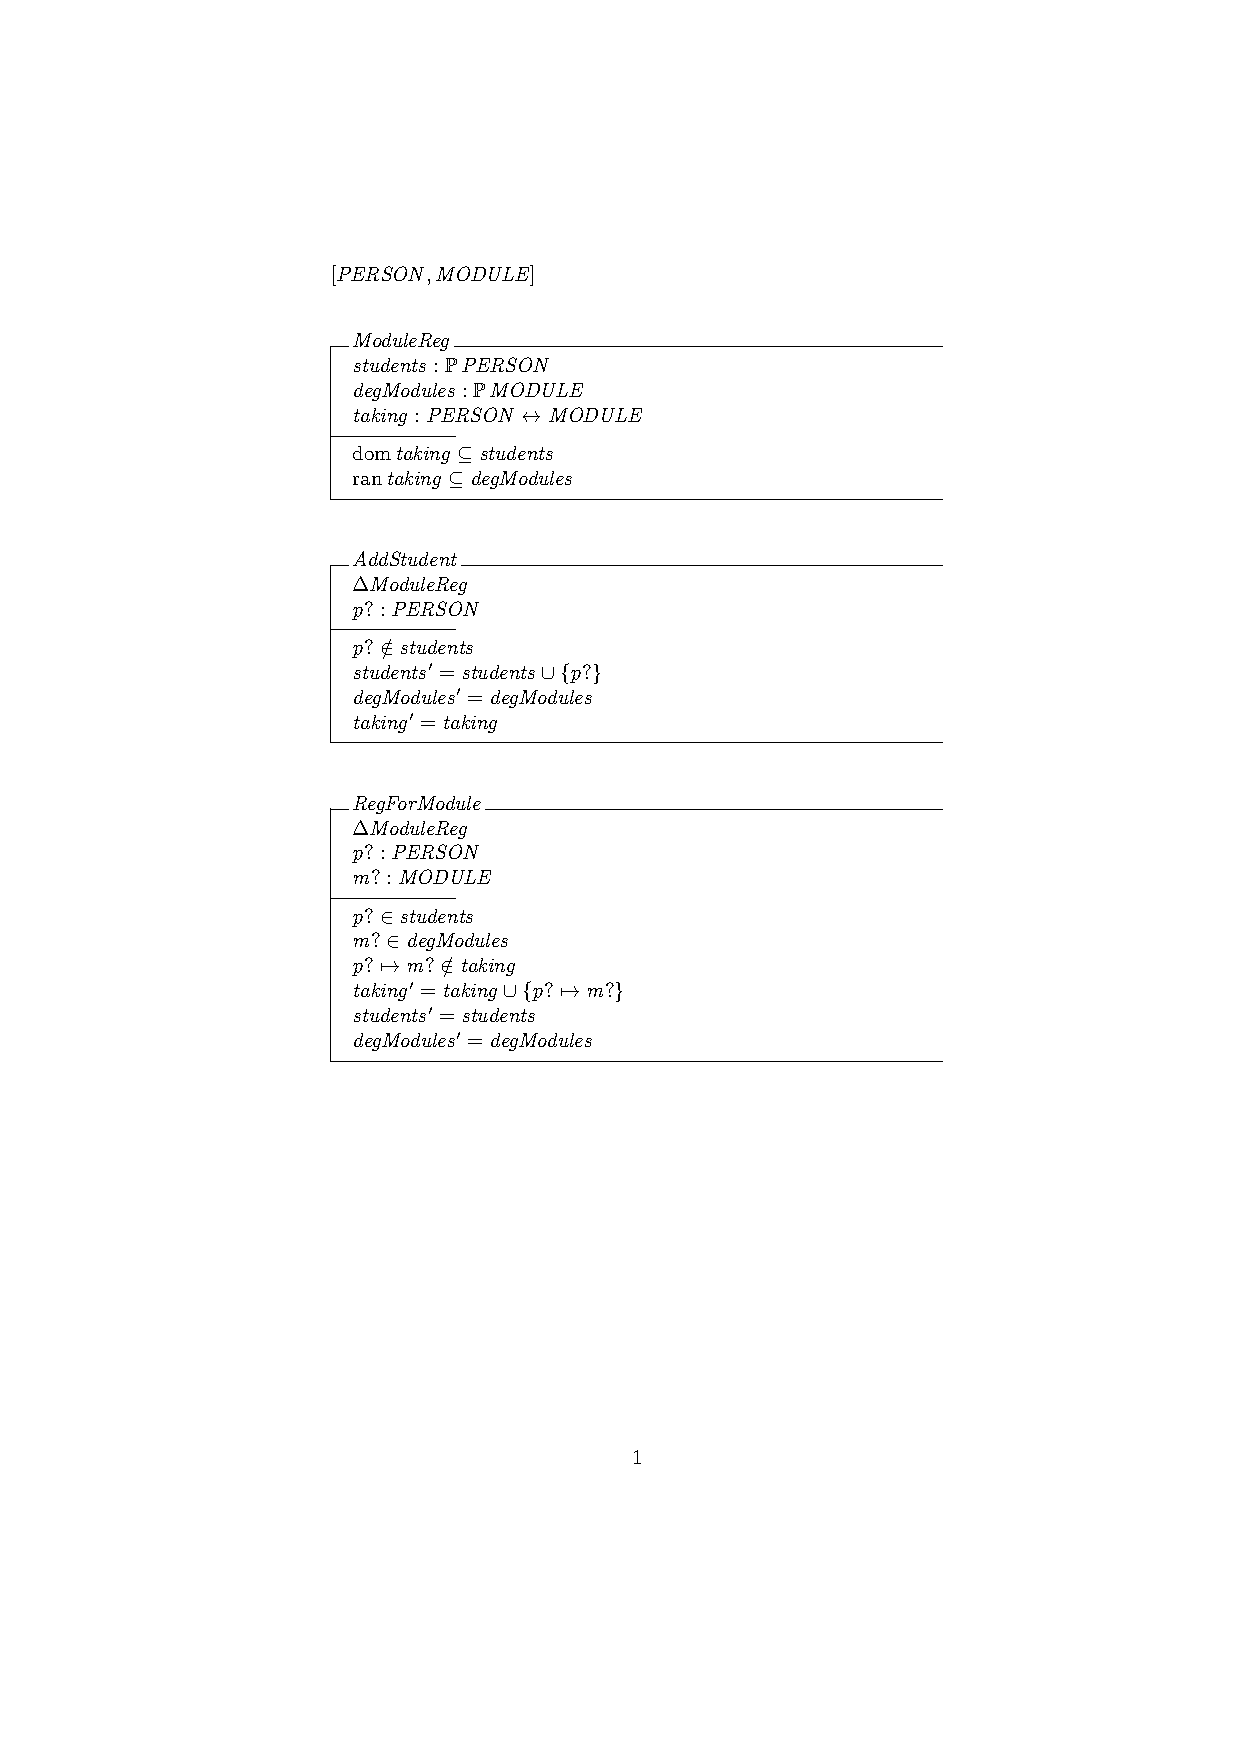
\includegraphics[trim=5cm 13cm 6 11cm]{examples/modulereg/0.pdf}}
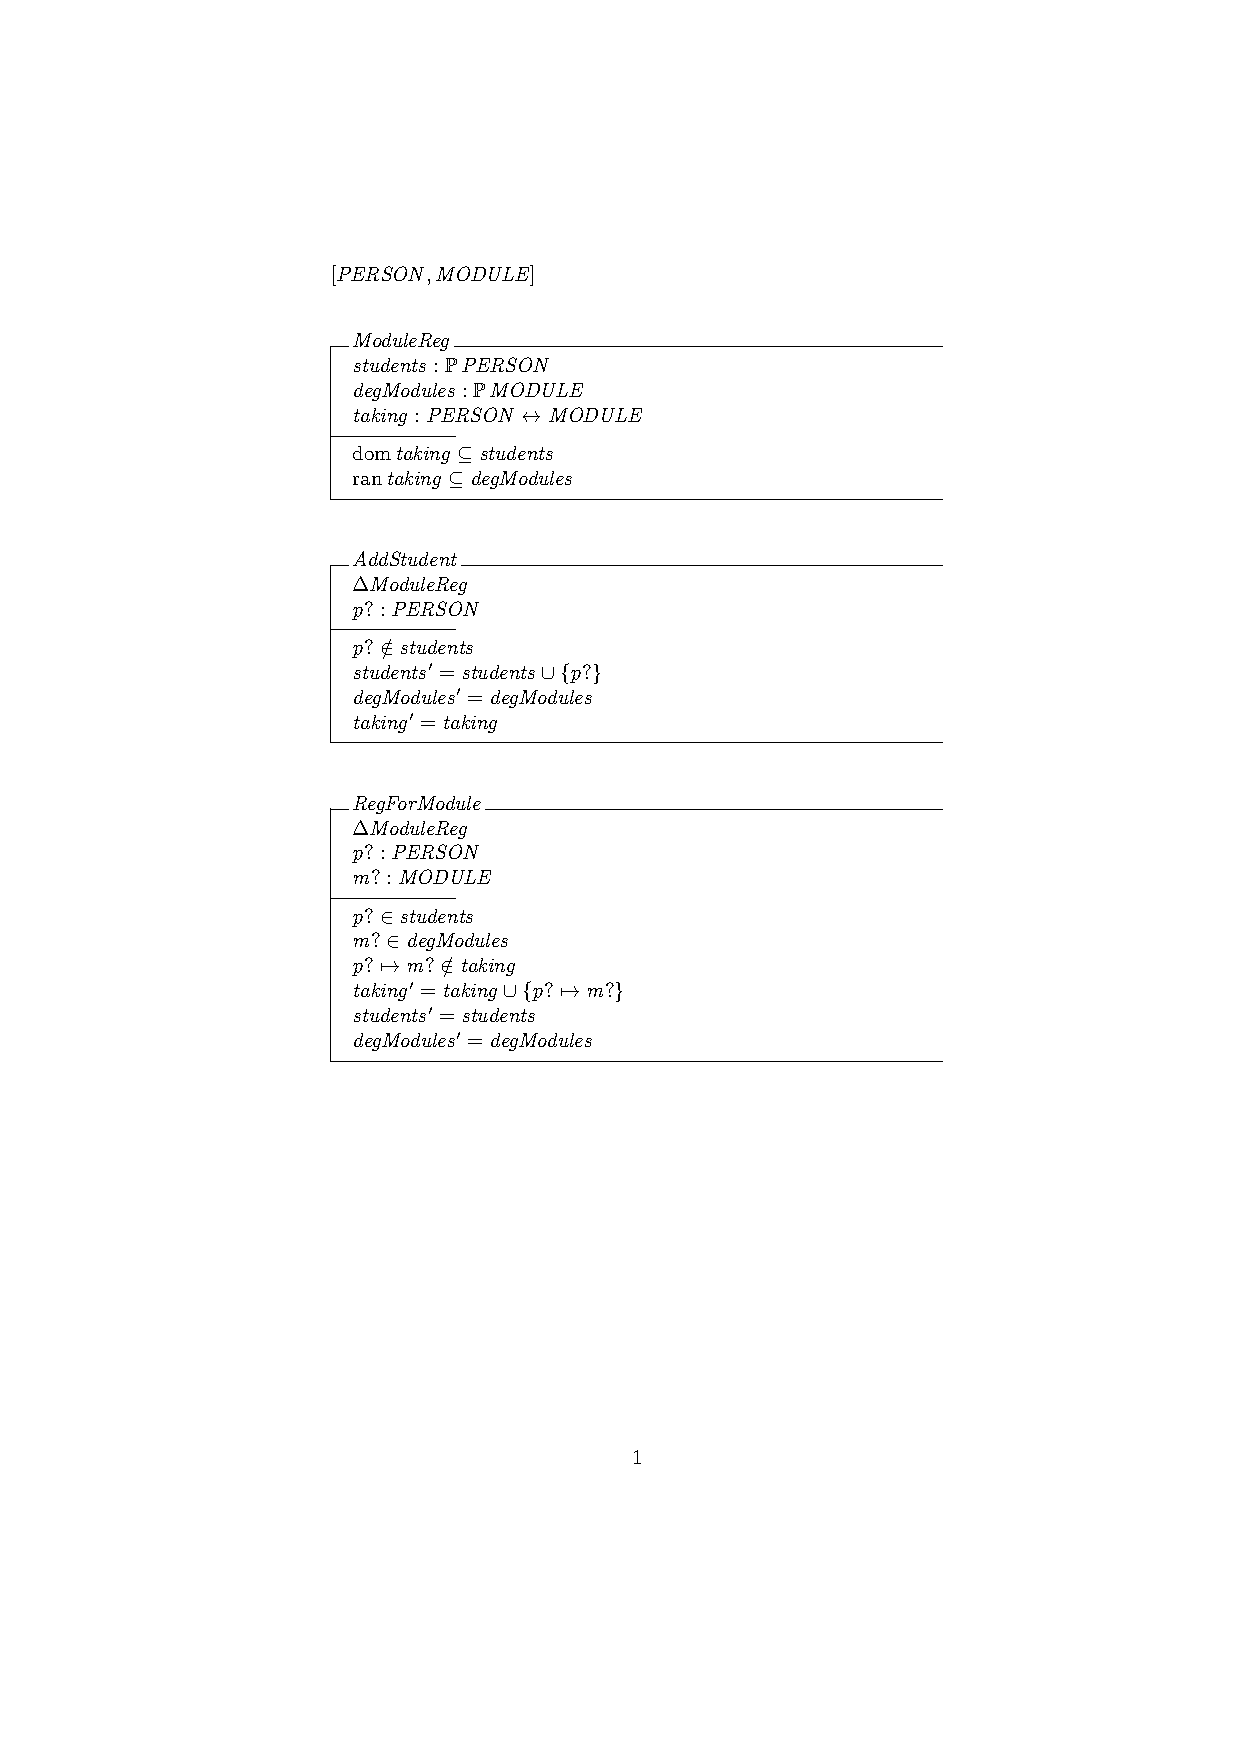
\includegraphics[clip, trim=5cm 11.5cm 10cm 5.5cm, width=1.00\textwidth]{examples/modulereg/0.pdf}
%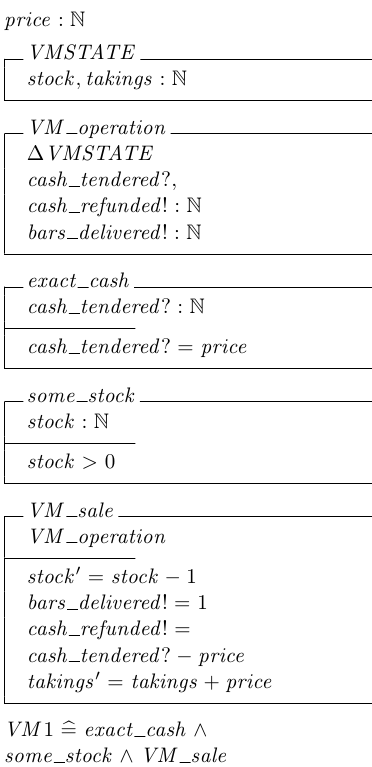
\includegraphics[scale=0.4]{Figures/fullexample/raw.png}
\vspace{-0.2in}
\caption{Part of a raw specification output. \label{fig:rawschemaout}}
\vspace{-0.2in}
\end{minipage}
\end{figure}


\section{Step 1\\ZCGa}

The user then goes to label the raw specification with the \gls{zcga} labels.
The labelled specification can be seen in figure \ref{fig:zcgaschema}. The words
highlighted in {\color{red}red} are the \gls{zcga} annotations done by the user
and the black text is the existing specification. Figure \ref{fig:zcgaschema}
outputting result can be seen in figure \ref{fig:zcgaschemaout}.

\begin{figure}[H]
\centering
\begin{minipage}{0.45\textwidth}
\centering
\begin{tiny}
\begin{BVerbatim}[commandchars=+\[\]]
\documentclass{article}
\usepackage{zmathlang}
\begin{document}
\begin{zed}
[+color[red]\set{]PERSON[+color[red]}], [+color[red]\set{]MODULE[+color[red]}]
\end{zed}
\begin{schema}{ModuleReg}
[+color[red]\text{\declaration{\set{]students[+color[red]}]:[+color[red]\expression{]\power
PERSON[+color[red]}}}]\\
[+color[red]\text{\declaration{\set{]degModules[+color[red]}]:[+color[red]\expression{]\power
MODULE[+color[red]}}}]\\
[+color[red]\text{\declaration{\set{]taking[+color[red]}]:[+color[red]\expression{]PERSON
\rel MODULE[+color[red]}}}]
\where
[+color[red]\text{\expression{\set{]\dom [+color[red]\set{]taking[+color[red]}}]
\subseteq [+color[red]\set{]students[+color[red]}}}]\\
[+color[red]\text{\expression{\set{]\ran [+color[red]\set{]taking[+color[red]}}]
\subseteq [+color[red]\set{]degModules[+color[red]}}}]
\end{schema}
\begin{schema}{AddStudent}
[+color[red]\text{]\Delta ModuleReg[+color[red]}]\\
[+color[red]\text{\declaration{\term{]p?[+color[red]}]:[+color[red]\expression{]PERSON[+color[red]}}}]\\
\where
[+color[red]\text{\expression{\term{]p?[+color[red]}] \notin
[+color[red]\set{]students[+color[red]}}}]\\
[+color[red]\text{\expression{\set{]students'[+color[red]}] =
[+color[red]\set{\set{]students[+color[red]}] \cup
[+color[red]\set{]\{[+color[red]\term{]p?[+color[red]}]\}[+color[red]}}}}]\\
[+color[red]\text{\expression{\set{]degModules'[+color[red]}] =
[+color[red]\set{]degModules[+color[red]}}}]\\
[+color[red]\text{\expression{\set{]taking'[+color[red]}] =
[+color[red]\set{]taking[+color[red]}}}]
\end{schema}
\begin{schema}{RegForModule}
[+color[red]\text{]\Delta ModuleReg[+color[red]}]\\
[+color[red]\text{\declaration{\term{]p?[+color[red]}]:
[+color[red]\expression{]PERSON[+color[red]}}}]\\
[+color[red]\text{\declaration{\term{]m?[+color[red]}]:
[+color[red]\expression{]MODULE[+color[red]}}}]
\where
[+color[red]\text{\expression{\term{]p?[+color[red]}] \in
[+color[red]\set{]students[+color[red]}}}]\\
[+color[red]\text{\expression{\term{]m?[+color[red]}] \in
[+color[red]\set{]degModules[+color[red]}}}]\\
[+color[red]\text{\expression{\term{\term{]p?[+color[red]}] \mapsto
[+color[red]\term{]m?[+color[red]}}] \notin
[+color[red]\set{]taking[+color[red]}}}]\\
[+color[red]\text{\expression{\set{]taking'[+color[red]}] =
[+color[red]\set{\set{]taking[+color[red]}] \cup
[+color[red]\set{]\{[+color[red]\term{\term{]p?[+color[red]}] \mapsto
[+color[red]\term{]m?[+color[red]}}]\}[+color[red]}}}}]\\
[+color[red]\text{\expression{\set{]students'[+color[red]}] =
[+color[red]\set{]students[+color[red]}}}]\\
[+color[red]\text{\expression{\set{]degModules'[+color[red]}] =
[+color[red]\set{]degModules[+color[red]}}}]
\end{schema}
\end{document}
\end{BVerbatim}
\end{tiny}
%\vspace{-0.2in}
\caption{Part of the raw schema.\label{fig:zcgaschema}}
%\vspace{-0.2in}
\end{minipage}\hfill
\begin{minipage}{0.45\textwidth}
\centering
\centering
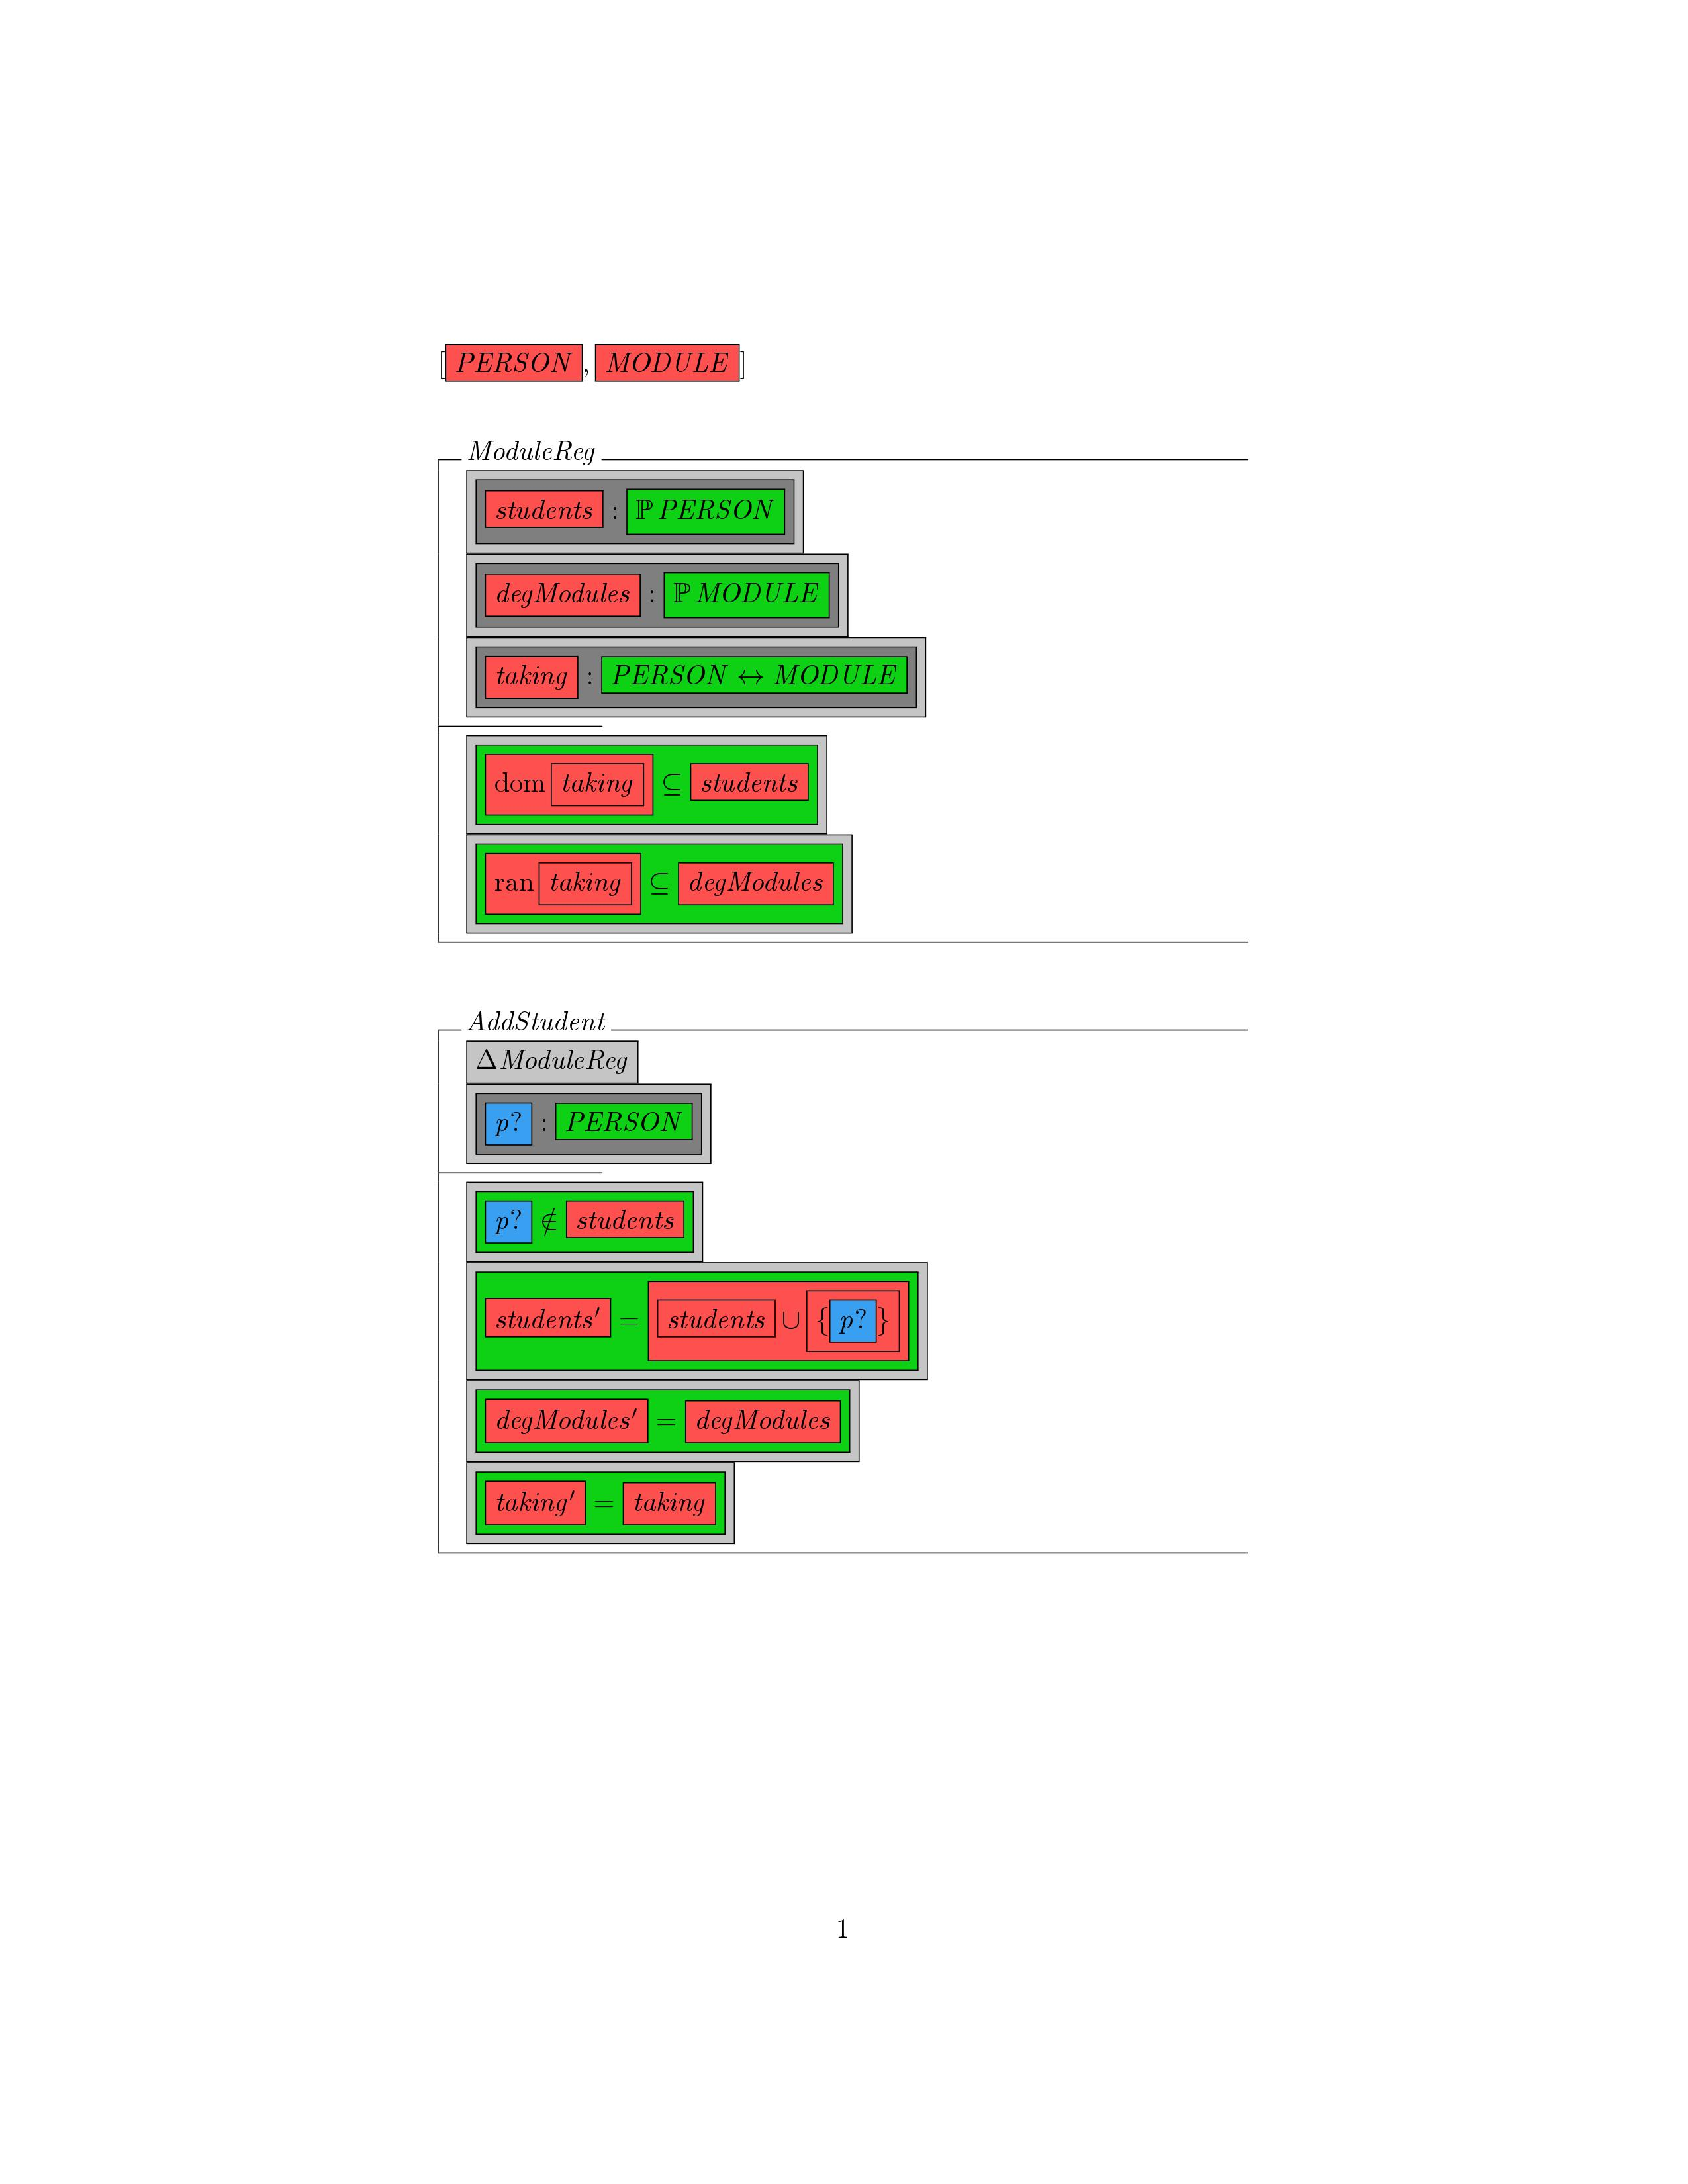
\includegraphics[scale=0.6, clip, trim=5.5cm 8cm 9.5cm 4cm, width=1.00\textwidth]{Figures/fullexample/1.jpg}
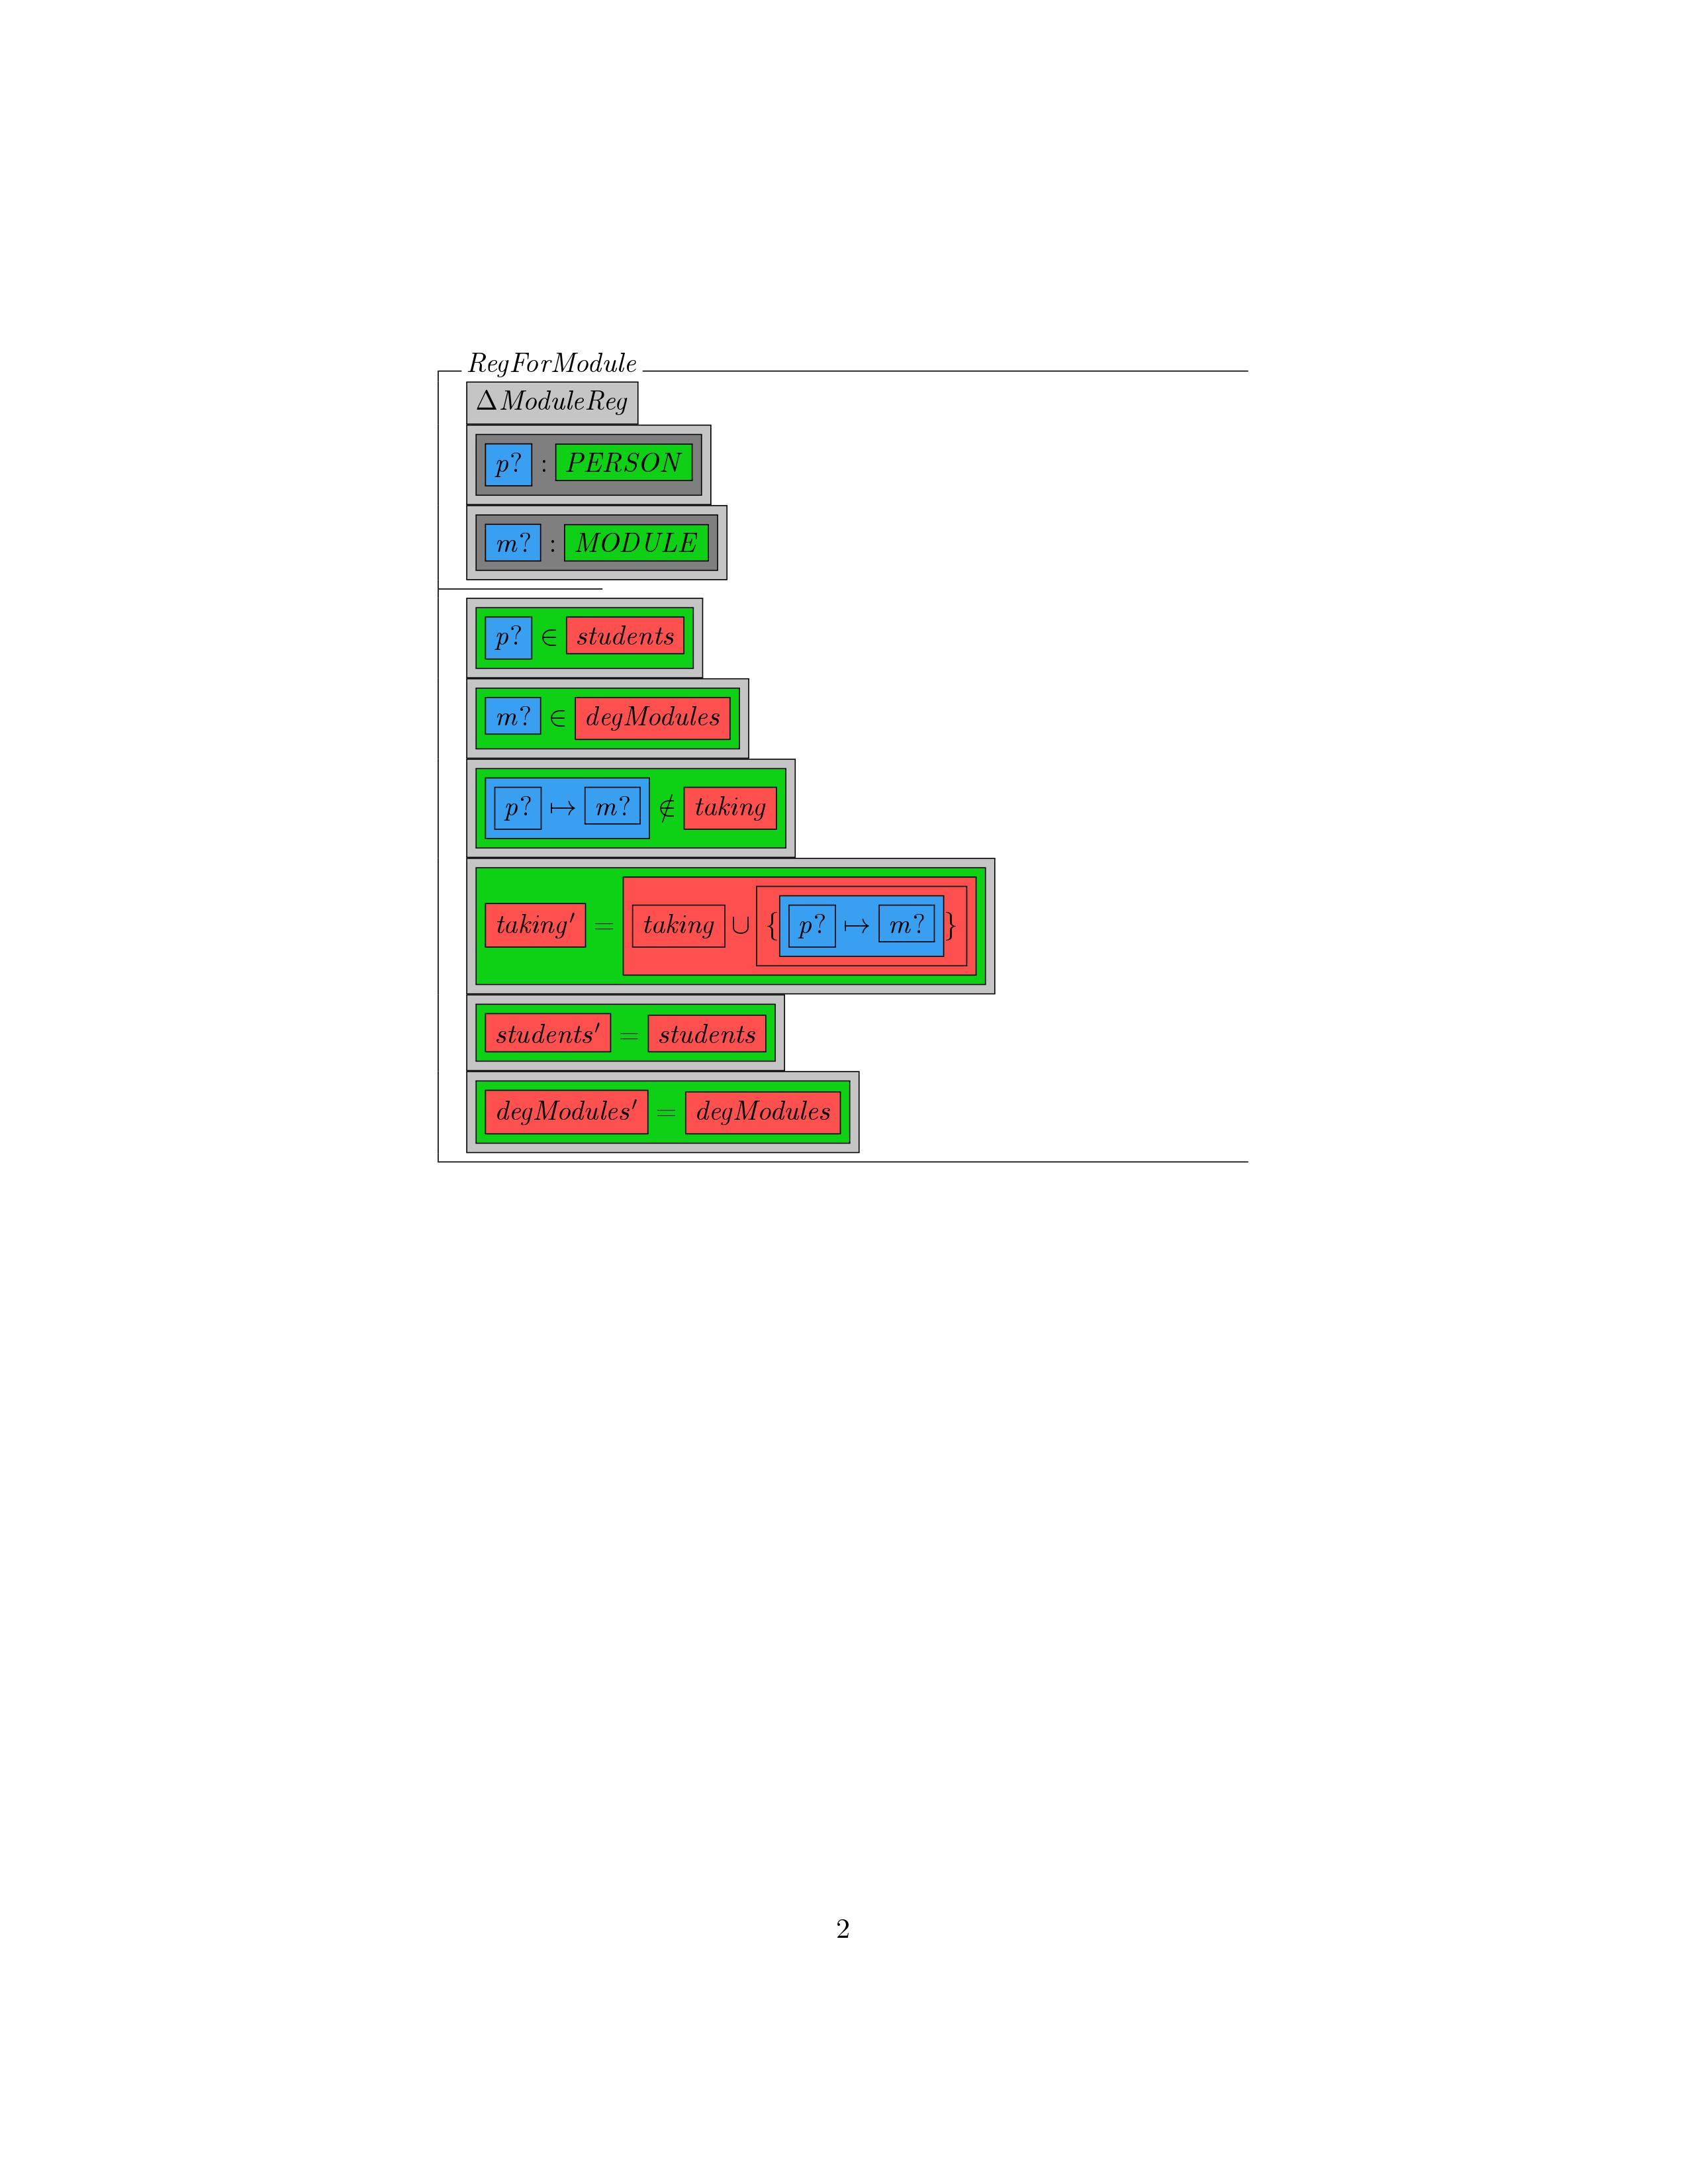
\includegraphics[scale=0.6, clip, trim=5.5cm 13cm 8.5cm 4cm, width=1.00\textwidth]{Figures/fullexample/2.jpg}
%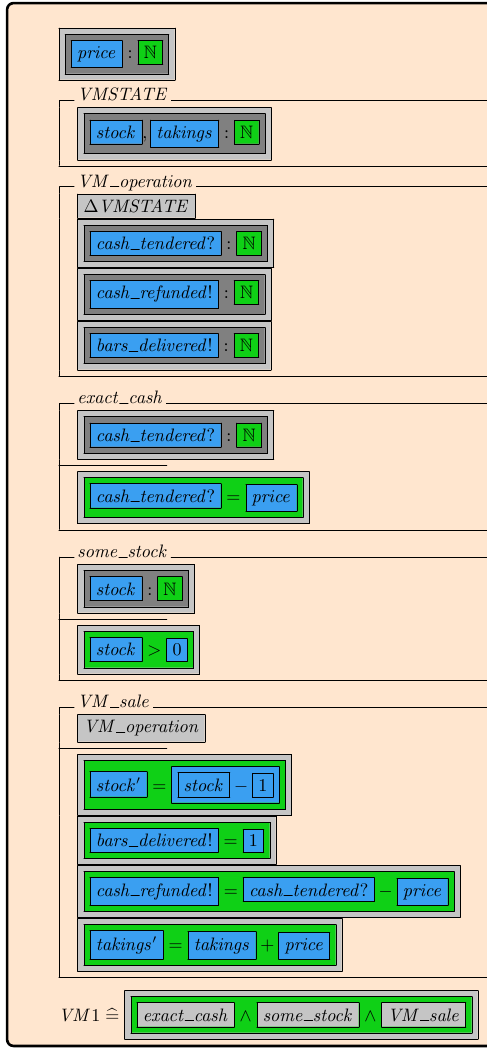
\includegraphics[scale=0.4]{Figures/fullexample/zcga.png}
\vspace{-0.3in}
\caption{Part of a ZCGa labelled specification output. \label{fig:zcgaschemaout}}
\end{minipage}
\end{figure}

After annotating we run it through the \gls{zcga} correctness checker. Figure
\ref{fig:zcgacorrect} shows the message which appears when the annotated
specification has been checked. 

\begin{figure}[H]
\centering
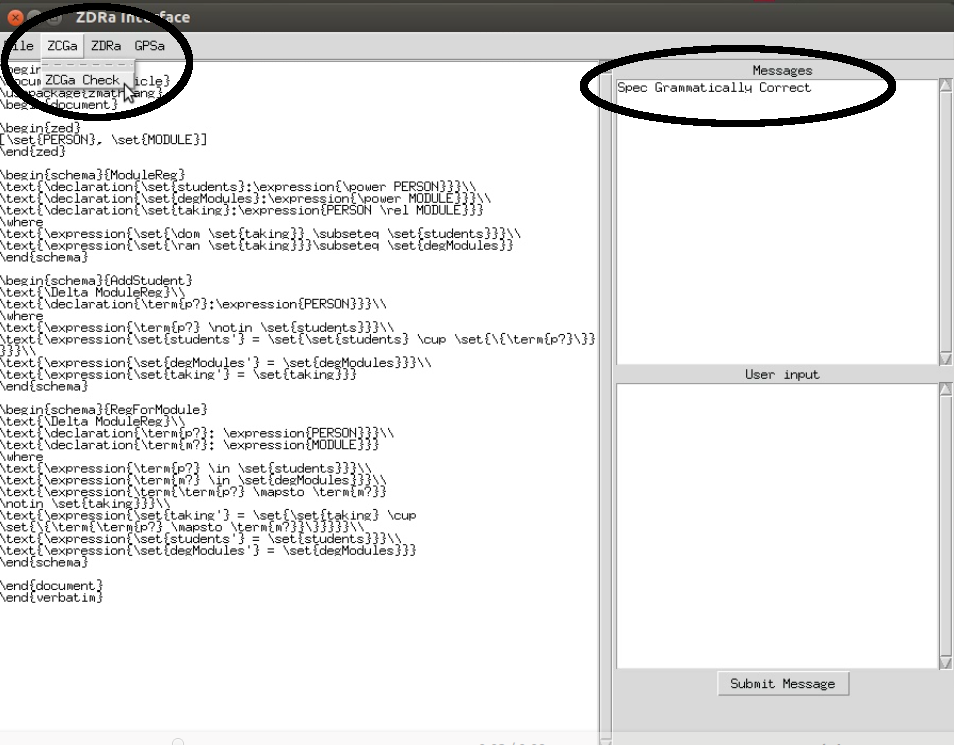
\includegraphics[scale=0.4]{Figures/fullexample/zcgacorrect.png}
\caption{Message which appears after running the ZCGa checker on our example. \label{fig:zcgacorrect}}
\end{figure}

\section{Step 2\\ZDRa}

Next the user can add \gls{zdra} relations to chunk parts of the specification
together and add relations to them. Figure \ref{fig:zdrazcgaAno} shows our
example labelled in \gls{zdra} annotations (in blue), the \gls{zcga} annotations
are in grey and existing specification in black. Figure \ref{fig:zdrazcgaout}
shows the compiled result.

\begin{figure}[H]
\vspace{-0.2in}
\centering
\begin{minipage}{0.45\textwidth}
\centering
\begin{tiny}
\begin{BVerbatim}[commandchars=+\[\]]
\documentclass{article}
\usepackage{zmathlang}
\begin{document}

[+color[blue]\dratheory{T1}{0.5}{]
\begin{zed}
[+color[gray]\set{]PERSON[+color[gray]}],
[+color[gray]\set{]MODULE[+color[gray]}]
\end{zed}

[+color[blue]\draschema{SS1}{]
\begin{schema}{ModuleReg}
[+color[gray]\text{\declaration{\set{]students[+color[gray]}]:[+color[gray]\expression{]\power
PERSON[+color[gray]}}}]\\
[+color[gray]\text{\declaration{\set{]degModules[+color[gray]}]:[+color[gray]\expression{]\power
MODULE[+color[gray]}}}]\\
[+color[gray]\text{\declaration{\set{]taking[+color[gray]}]:[+color[gray]\expression{]PERSON
\rel MODULE[+color[gray]}}}]
\where
[+color[blue]\draline{SI1}{] [+color[gray]\text{\expression{\set{]\dom
[+color[gray]\set{]taking[+color[gray]}}] \subseteq
[+color[gray]\set{]students[+color[gray]}}}]\\
[+color[gray]\text{\expression{\set{]\ran
[+color[gray]\set{]taking[+color[gray]}}] \subseteq
[+color[gray]\set{]degModules[+color[gray]}}}][+color[blue]}]
\end{schema}[+color[blue]}]

[+color[blue]\requires{SS1}{SI1}]

[+color[blue]\draschema{CS1}{]
\begin{schema}{AddStudent}
[+color[gray]\text{]\Delta ModuleReg[+color[gray]}]\\
[+color[gray]\text{\declaration{\term{]p?[+color[gray]}]:[+color[gray]\expression{]PERSON[+color[gray]}}}]\\
\where
[+color[blue]\draline{PRE1}{]
[+color[gray]\text{\expression{\term{]p?[+color[gray]}] \notin
[+color[gray]\set{]students[+color[gray]}}}][+color[blue]}]\\
[+color[blue]\draline{PO1}{]
[+color[gray]\text{\expression{\set{]students'[+color[gray]}] =
[+color[gray]\set{\set{]students[+color[gray]}] \cup
[+color[gray]\set{]\{[+color[gray]\term{]p?[+color[gray]}]\}[+color[gray]}}}}]\\
[+color[gray]\text{\expression{\set{]degModules'[+color[gray]}] =
[+color[gray]\set{]degModules[+color[gray]}}}]\\
[+color[gray]\text{\expression{\set{]taking'[+color[gray]}] =
[+color[gray]\set{]taking[+color[gray]}}}][+color[blue]}]
\end{schema}[+color[blue]}]

[+color[blue]\requires{CS1}{PRE1}] [+color[blue]\allows{PRE1}{PO1}]
[+color[blue]\uses{CS1}{SS1}]

[+color[blue]\draschema{CS2}{]
\begin{schema}{RegForModule}
[+color[gray]\text{]\Delta ModuleReg[+color[gray]}]\\
[+color[gray]\text{\declaration{\term{]p?[+color[gray]}]:
[+color[gray]\expression{]PERSON[+color[gray]}}}]\\
[+color[gray]\text{\declaration{\term{]m?[+color[gray]}]:
[+color[gray]\expression{]MODULE[+color[gray]}}}]
\where

\end{document}
\end{BVerbatim}
\end{tiny}
%\vspace{-0.18in}
\caption{An example of a specification labelled in \gls{zcga} and \gls{zdra}.).\label{fig:zdrazcgaAno}}
%\vspace{-0.2in}
\end{minipage}\hfill
\begin{minipage}{0.45\textwidth}
\centering
\begin{tiny}
\begin{BVerbatim}[commandchars=+\[\]]
[+color[blue]\draline{PRE2}{]
[+color[gray]\text{\expression{\term{]p?[+color[gray]}] \in
[+color[gray]\set{]students[+color[gray]}}}]\\
[+color[gray]\text{\expression{\term{]m?[+color[gray]}] \in
[+color[gray]\set{]degModules[+color[gray]}}}]\\
[+color[gray]\text{\expression{\term{\term{]p?[+color[gray]}] \mapsto
[+color[gray]\term{]m?[+color[gray]}}] \notin
[+color[gray]\set{]taking[+color[gray]}}}][+color[blue]}]\\
[+color[blue]\draline{PO2}{]
[+color[gray]\text{\expression{\set{]taking'[+color[gray]}] =
[+color[gray]\set{\set{]taking[+color[gray]}] \cup
[+color[gray]\set{]\{[+color[gray]\term{\term{]p?[+color[gray]}] \mapsto
[+color[gray]\term{]m?[+color[gray]}}]\}[+color[gray]}}}}]\\
[+color[gray]\text{\expression{\set{]students'[+color[gray]}] =
[+color[gray]\set{]students[+color[gray]}}}]\\
[+color[gray]\text{\expression{\set{]degModules'[+color[gray]}] =
[+color[gray]\set{]degModules[+color[gray]}}}][+color[blue]}]
\end{schema}[+color[blue]}] [+color[blue]}]


\end{BVerbatim}
\end{tiny}
%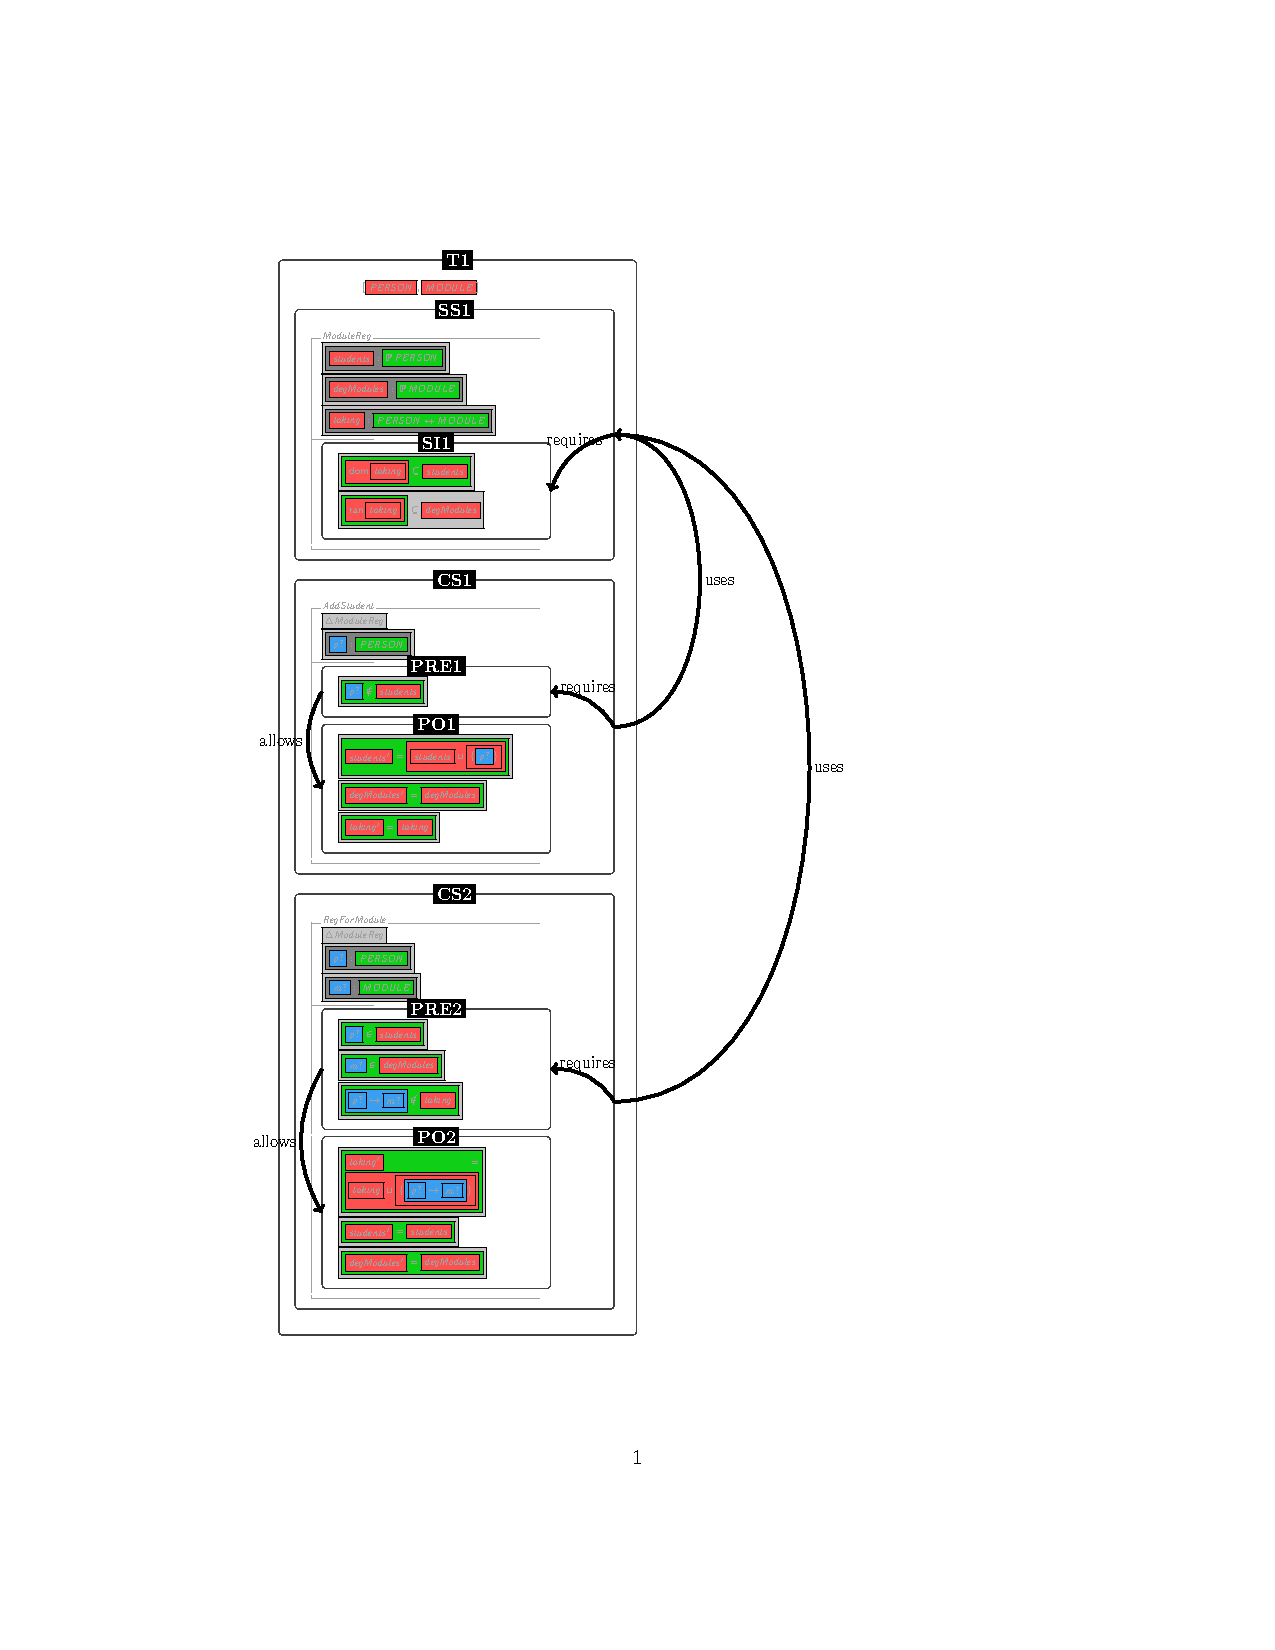
\includegraphics[scale=1, clip, trim=2cm 3cm 2cm 3cm, width=1.00\textwidth]{Figures/fullexample/1n2.pdf}
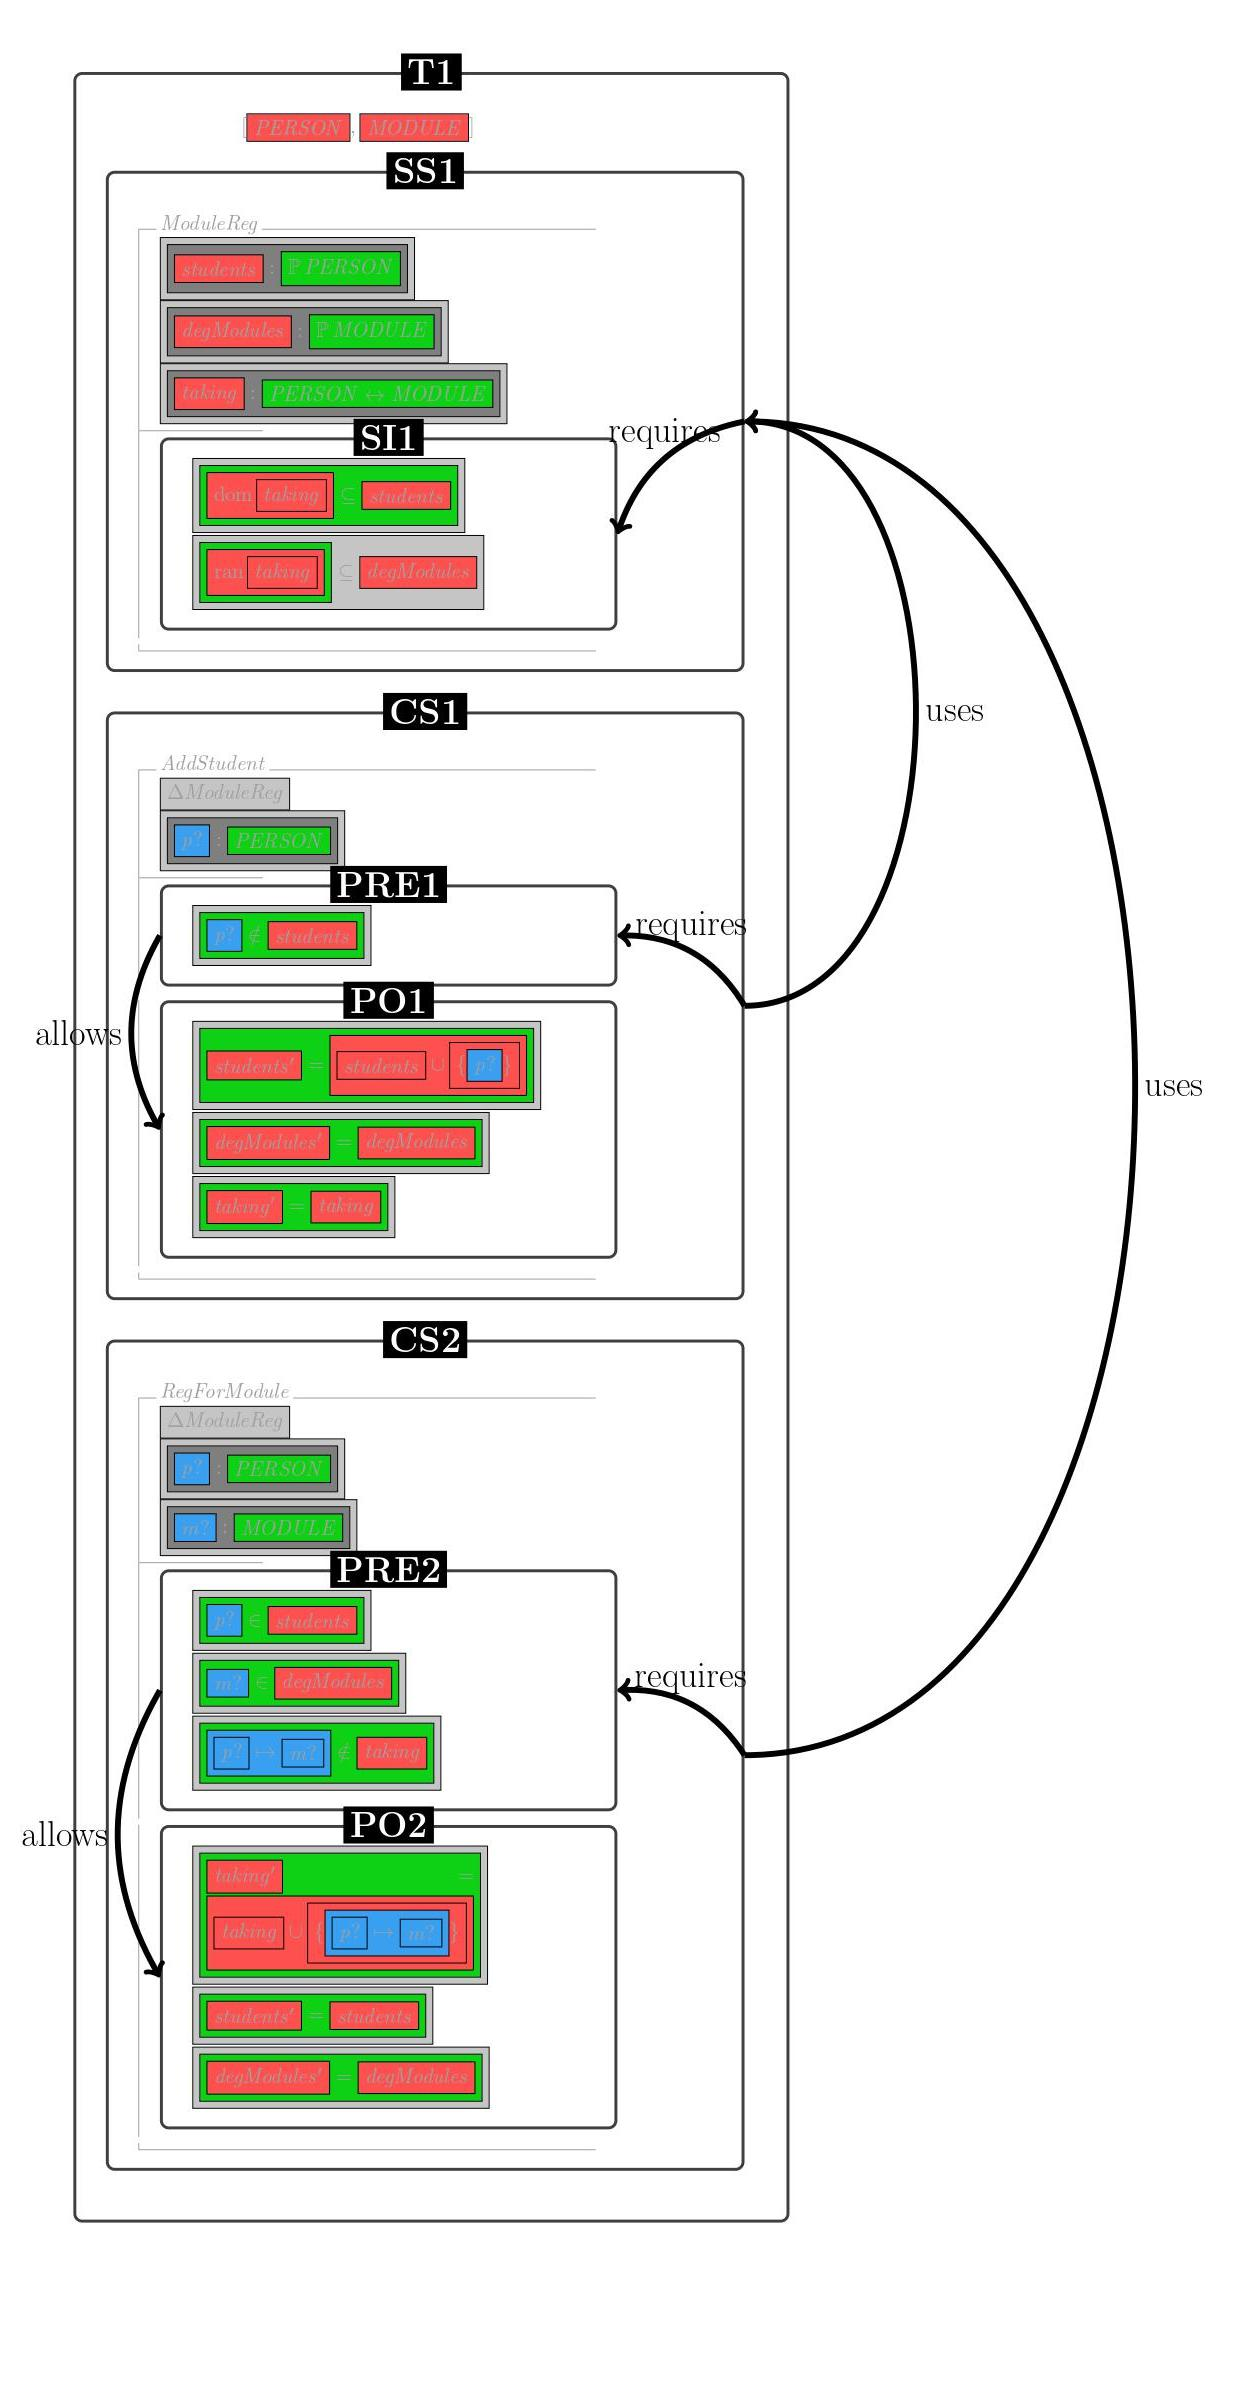
\includegraphics[scale=0.8]{Figures/fullexample/1n2.jpg}
%\vspace{-0.18in}
\caption{An example of a specification output labelled in \gls{zcga} and \gls{zdra}.).\label{fig:zdrazcgaout}}
%\vspace{-0.2in}
\end{minipage}
\end{figure}

After annotating our example in \gls{zdra} labels we can then run our
specification through the \gls{zdra} checker. Figure \ref{fig:zdracorrect} shows
the message which appears after we check our example with \gls{zdra}.

\begin{figure}[H]
\centering
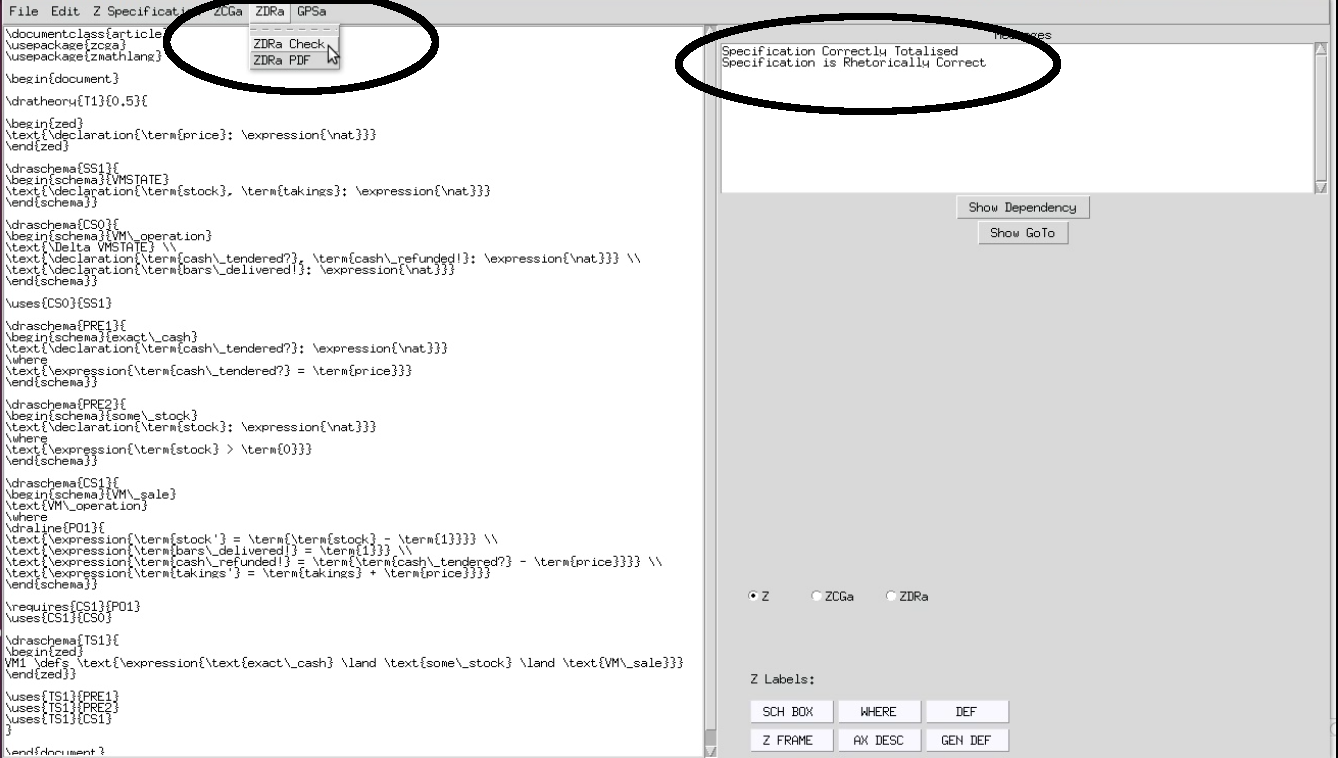
\includegraphics[scale=0.3]{Figures/fullexample/zdracorrect.png}
\caption{Message which appears after running the ZDRa checker on our example. \label{fig:zdracorrect}}
\end{figure}

\section{Step 2.5\\Graphs}

Since the example is \gls{zdra} correct the two graphs shown in figures
\ref{fig:depexample} and \ref{fig:gotoexample} are automatically produced and
saved on the users computer.

\begin{figure}[H]
\centering
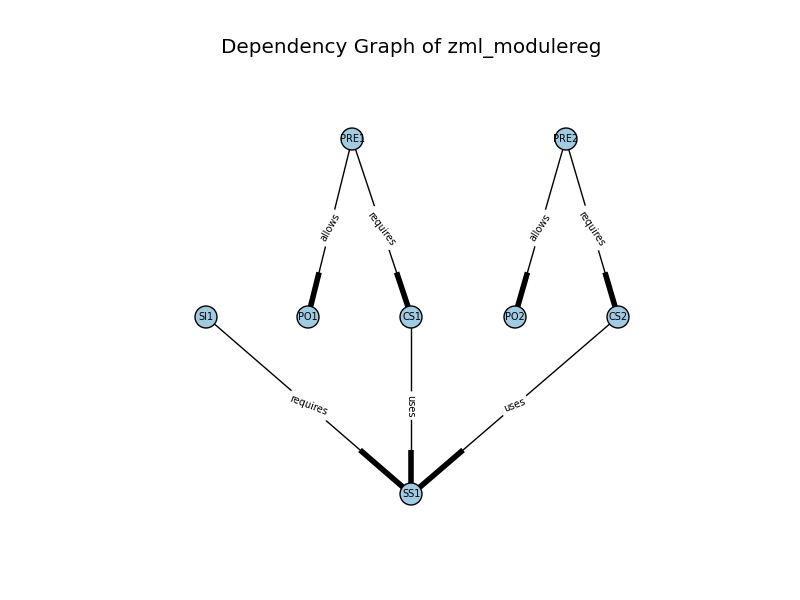
\includegraphics[scale=0.7]{Figures/fullexample/dp_fullexample.png}
\caption{Dependency graph automatically generated from the ZDRa for our example. \label{fig:depexample}}
\end{figure}

\begin{figure}[H]
\centering
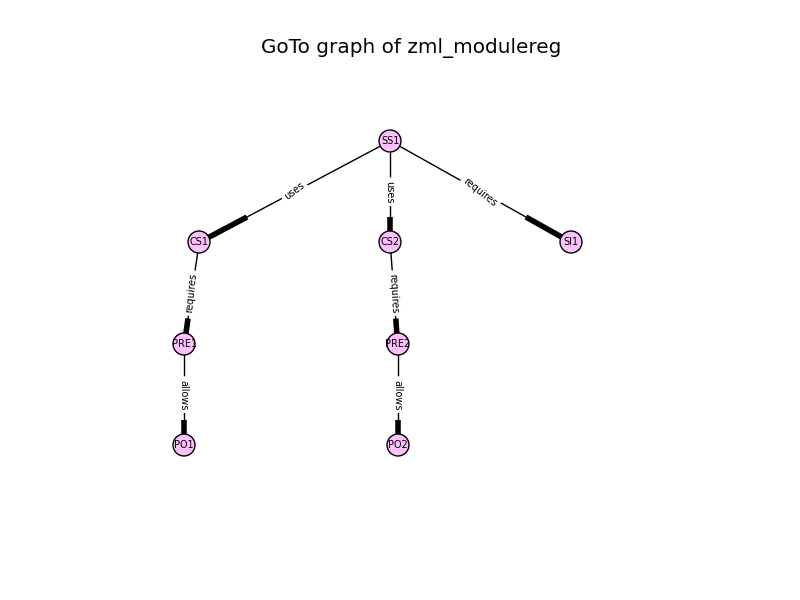
\includegraphics[scale=0.7]{Figures/fullexample/goto_fullexample.jpg}
\caption{GoTo graph automatically generated from the ZDRa for our example. \label{fig:gotoexample}}
\end{figure}

\section{Skeletons}

The skeletons are automatically generated if the specification passes the
\gls{zcga} and \gls{zdra} check.

\subsection{Step 3\\General Proof Skeleton}

We can generate a general proof skeleton which prints out the \gls{zdra} name
and the instances they should be converted to when inputting into any theorem
prover. If the specification is \gls{zdra} correct we can then generate the
\gls{gpsa} by clicking on the \gls{gpsa} menu in the interface (figure
\ref{fig:gpsabutton}).

\begin{figure}[H]
\centering
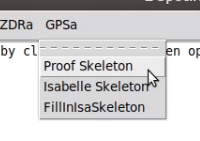
\includegraphics[scale=1]{Figures/fullexample/proofskelbutton.png}
\caption{The GPSa button allows the user to generate the general proof skeleton. \label{fig:gpsabutton}}
\end{figure}

The GPSa can be created after a specification has been annotated with ZDRa. The GPSa is what orders the specification 
logically to put into a theorem prover. Steps 4, 5 and 6 will need to be created after the GPSa. Step 4 will uses the skeleton 
created in step 3 and ZCGa annotations created in step 2 to create the Isabelle skeleton. The Isabelle skeleton in
step 4 requires ZCGa annotations and the GPSa to be complete. Without the GPSa the logical order of the specification may not be correct
e.g. there may be some changeSchemas used which haven't been created yet. Without the ZCGa the some variables may be used which havn't been 
declared and therefore will not pass through Isabelle.

Figure \ref{fig:gpsaFullexample} shows the general proof skeleton which was
generated for our example. Note all instances but the last 2 are actual
instances labelled by the user. Since there are 2 instances where there could be
a change in state (CS1 and CS2) then there are 2 proof obligations added to the
\gls{gpsa} (L1\_CS2 and L2\_CS1).

\begin{figure}[H]
\centering
\begin{scriptsize}
\begin{BVerbatim}
stateSchema SS1 stateInvariants SI1 changeSchema CS2 precondition PRE2
changeSchema CS1 precondition PRE1 postcondition PO2 postcondition PO1 lemma
L1_(CS2) lemma L2_(CS1) 
\end{BVerbatim}
\end{scriptsize}
\caption{General proof skeleton. \label{fig:gpsaFullexample}}
\end{figure}

\subsection{Step 4\\Isabelle Skeleton}

From \gls{gpsa}, the ZMathLang program can automatically generate an Isabelle
Skeleton. The user can do this by clicking on the \gls{gpsa} menu on the
interface then clicking `\texttt{Isabelle Skeleton}' shown in figure
\ref{fig:isabutton}.

\begin{figure}[H]
\centering
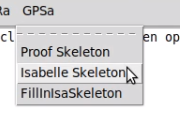
\includegraphics[scale=1]{Figures/fullexample/isaskelbutton.png}
\caption{The Isabelle skeleton button allows the user to generate an Isabelle skeleton of their specification. \label{fig:isabutton}}
\end{figure}

 The Isabelle skeleton consists of the information generated in the general
 proof skeleton along with the environment to begin an Isabelle theory. It
 contains comments in between \verb|(* .. *)| parenthesis to show the parts which
 need to be filled in either by using the \gls{zcga} document or by the user.
 Figure \ref{fig:isaFullexample} shows the automatically generated Isabelle
 skeleton for our \texttt{modulereg} example.

\begin{figure}[H]
\centering
\begin{scriptsize}
\begin{BVerbatim}
theory gpsaModuleReg imports Main begin (*DATATYPES*) record SS1 = (*DECLARATIONS*)
locale 1n2 = fixes (*GLOBAL DECLARATIONS*) assumes SI1 begin definition CS2 ::
"(*CS2_TYPES*) => bool" where "CS2 (*CS2_VARIABLES*) == (PRE2) \<and> (PO2)"
definition CS1 :: "(*CS1_TYPES*) => bool" where "CS1 (*CS1_VARIABLES*) == (PRE1)
\<and> (PO1)"

lemma CS2_L1: "(\<exists> (*CS2_VARIABLESANDTYPES*). (PRE2) \<and> (PO2) \<and>
(SI1) \<and> (SI1'))" sorry lemma CS1_L2: "(\<exists> (*CS1_VARIABLESANDTYPES*).
(PRE1) \<and> (PO1) \<longrightarrow> ((SI1) \<and> (SI1')))" sorry end end

\end{BVerbatim}
\end{scriptsize}
\caption{Isabelle proof skeleton. \label{fig:isaFullexample}}
\end{figure}

%\begin{figure}[H]
%\centering
%\begin{minipage}{0.45\textwidth}
%\centering
%\begin{scriptsize}
%\begin{BVerbatim}
%theory gpsa1n2 imports Main begin (*DATATYPES*) record SS1 = (*DECLARATIONS*)
%locale 1n2 = fixes (*GLOBAL DECLARATIONS*) assumes SI1 begin definition CS2 ::
%"(*CS2_TYPES*) => bool" where "CS2 (*CS2_VARIABLES*) == (PRE2) \<and> (PO2)"
%definition CS1 :: "(*CS1_TYPES*) => bool" where "CS1 (*CS1_VARIABLES*) == (PRE1)
%\<and> (PO1)"
%\end{BVerbatim}
%\end{scriptsize}
%\end{minipage}\hfill
%\begin{minipage}{0.45\textwidth}
%\begin{scriptsize}
%\begin{BVerbatim}
%lemma CS2_L1: "(\<exists> (*CS2_VARIABLESANDTYPES*). (PRE2) \<and> (PO2) \<and>
%(SI1) \<and> (SI1'))" sorry lemma CS1_L2: "(\<exists> (*CS1_VARIABLESANDTYPES*).
%(PRE1) \<and> (PO1) \<longrightarrow> ((SI1) \<and> (SI1')))" sorry end end
%\end{BVerbatim}
%\end{scriptsize}
%\end{minipage}
%\caption{Isabelle proof skeleton. \label{fig:isaFullexample}}
%\end{figure}

\subsection{Step 5\\Isabelle Skeleton Filled in}

Using the \gls{zcga} annotated document and the Isabelle skeleton described in
the previous section. The user can then automatically fill in the missing
information which is needed between the comment parenthesis \verb|(* ...*)|.
This is the final step which is automated by the program and the user can click
on the \gls{gpsa} button on the main menu bar in the interface and then click on
`\texttt{FillInIsa Skeleton}' in the sub menu (shown in figure
\ref{fig:fillinisa}).

\begin{figure}[H]
\centering
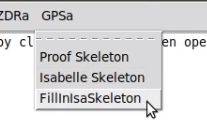
\includegraphics[scale=1]{Figures/fullexample/fillinisabutton.png}
\caption{The "FillInIsa Skeleton" button allows the user to fill in the skeleton they previously created. \label{fig:fillinisa}}
\end{figure}

Figure \ref{fig:fillinFullexample} shows our example with a filled in Isabelle
skeleton. It is important to note that the program also changes some of the
syntax from \LaTeX{} to Isabelle so that it is fully parsable by Isabelle.
We have used the rules described in section \ref{sec:zcga2fillin} to fill in the Isabelle
 skeleton with the ZCGa annotations.

\begin{figure}[H]
\centering
\begin{minipage}{0.45\textwidth}
\centering
\begin{scriptsize}
\begin{BVerbatim}
theory gpsaModuleReg imports Main 

begin typedecl PERSON typedecl MODULE

record ModuleReg = STUDENTS :: " PERSON set"
DEGMODULES :: " MODULE set" TAKING
:: "(PERSON * MODULE) set"

locale gpsaModuleReg = fixes students :: 
" PERSON set" and degModules :: "
MODULE set" and taking :: "(PERSON * MODULE) set"
 assumes "Domain taking
\<subseteq> students" and 
"Range taking \<subseteq> degModules" begin

definition RegForModule :: 
"ModuleReg \<Rightarrow> ModuleReg \<Rightarrow>
PERSON \<Rightarrow> MODULE => MODULE set 
\<Rightarrow> PERSON set \<Rightarrow>
(PERSON * MODULE) set \<Rightarrow> bool" where 
"RegForModule modulereg
modulereg' p m degModules' students' taking' == 
(p \<in> students) \<and> (m
\<in> degModules) \<and> ((p, m) \<notin> taking) 
\<and> (taking' = taking\<union> {(p, m)}) \<and> 
(students' = students) 
\<and> (degModules' =degModules)"

definition AddStudent :: "ModuleReg \<Rightarrow> 
ModuleReg => PERSON
\<Rightarrow>  MODULE set \<Rightarrow> PERSON set 
\<Rightarrow> (PERSON *
MODULE) set \<Rightarrow> bool" where "AddStudent 
modulereg modulereg' p
degModules' students' taking' == ((p \<notin> students) 
\<and> (students' =
students \<union> {(p)}) 
\end{BVerbatim}
\end{scriptsize}
\end{minipage}\hfill
\begin{minipage}{0.45\textwidth}
\begin{scriptsize}
\begin{BVerbatim}
\<and> (degModules' = degModules) \<and> 
(taking' = taking))"

lemma RegForModule_L1: 
"(\<exists> degModules:: MODULE set. 
\<exists> students
:: PERSON set. \<exists> taking :: 
(PERSON * MODULE) set. \<exists> p :: PERSON.
\<exists> degModules':: MODULE set. 
\<exists> students' :: PERSON set. \<exists>
taking' :: (PERSON * MODULE) set. 
\<exists> m :: MODULE. ((p \<in> students)
\<and> (m \<in> degModules) \<and> ((p, m) 
\<notin> taking) \<and> (taking' =
taking \<union> {(p, m)}) \<and> 
(students' = students) 
\<and> (degModules' =
degModules)) \<longrightarrow> ((Domain taking 
\<subseteq> students) \<and>
(Range taking \<subseteq> degModules) \<and> 
(Domain taking' \<subseteq>
students') \<and> (Range taking' 
\<subseteq> degModules')))" sorry

lemma AddStudent_L2: 
"(\<exists> degModules:: MODULE set. 
\<exists> students ::
PERSON set. \<exists> taking :: 
(PERSON * MODULE) set. 
\<exists> p :: PERSON.
\<exists> degModules':: MODULE set. 
\<exists> students' :: PERSON set. \<exists>
taking' :: (PERSON * MODULE) set. 
( (students' = students \<union> {(p)}) \<and>
(degModules' = degModules) \<and> 
(taking' = taking)) 
\<longrightarrow ((Domain
taking \<subseteq> students) \<and> 
(Range taking \<subseteq> degModules) \<and>
(Domain taking' \<subseteq> students') 
\<and> (Range taking' \<subseteq>
degModules')))" sorry end end
\end{BVerbatim}
\end{scriptsize}
\end{minipage}
\caption{Filled In proof skeleton. \label{fig:fillinFullexample}}
\end{figure}

Figure \ref{fig:fillinFullexample} shows the original specification we started
with in step 0 in Isabelle syntax. It is important to the reader to note that we
have come this far without the user knowing any Isabelle at all. In our example
we have 2 existing lemma's to prove to check the consistency of the
specification. That is the state before \texttt{RegForModule} (PRE2), \emph{and}
the state after \texttt{RegforModule} (PO2), \emph{implies}
\texttt{stateInvariants} (SI1), \emph{and} the \texttt{stateInvariants'} (SI1')
is true. So the precondition and postcondition imply that the stateInvariants
and stateInvariants prime hold. The same goes for the \texttt{AddStudent}
operation. When the skeleton is Filled in the \gls{zmath} is unable to prove the
lemma's automatically and it is up to the user to do this (explained in the next
section). However at this stage \gls{zmath} puts the Isar command
`\texttt{sorry}' as to ignore the lemma and act as if it was proven.

In this case the new "Lemmas" are added to the end of the specification at random.
For this specification it doesn't matter which lemma comes first (RegForModule\_L1 or AddStudent\_L2)
as the schemas \texttt{RegForModule} and \texttt{AddStudent} are independent of eachother
and one does not `\textit{use}' the other. If we did have a changeSchema which did use another changeSchema
then this would have to be annotated in the zDRa and therefore the order would matter when the lemmas are produced.


\section{Step 6\\Full Proof}

The next part is to prove any existing lemmas from the filled in Isabelle
Skeleton or add new lemma's to prove safety properties about the specification.
However, this final stage is difficult to automate with \gls{zmath} as everyone
has different properties they wish to prove and all specification are different
themselves. So the final step will need some theorem prover knowledge, but not
as much as translating the specification and proving it in one step as the
specification is already put into the theorem prover syntax. In this case the
user may wish to use theorem prover tools which already exist such as
Sledgehammer \cite{sledgehammer} to help them prove the properties. An example
is shown in figure \ref{fig:propertyproof} the proof obligations being proven by
hand for the \texttt{modulereg} specification.

\begin{figure}[H]
\centering
\begin{minipage}{0.45\textwidth}
\centering
\begin{scriptsize}
 

\begin{BVerbatim}[commandchars=+\[\]] 
lemma RegForModule_L1: "(\<exists>
degModules:: MODULE set. \<exists> students ::
 PERSON set. \<exists> taking ::
(PERSON * MODULE) set. \<exists> p :: PERSON. 
\<exists> degModules':: MODULE
set. \<exists> students' :: PERSON set. 
\<exists> taking' :: (PERSON * MODULE)
set. \<exists> m :: MODULE. ((p \<in> students) 
\<and> (m \<in> degModules)
\<and> ((p, m) \<notin> taking) \<and> 
(taking' = taking \<union> {(p, m)})
\<and> (students' = students) \<and> 
(degModules' = degModules))
\<longrightarrow> ((Domain taking 
\<subseteq> students)  \<and> (Range taking
\<subseteq> degModules) \<and> (Domain taking' 
\<subseteq> students') \<and>
(Range taking' \<subseteq> degModules')))"

[+color[red]by (smt Domain_empty Domain_insert] 
[+color[red]Range.intros
Range_empty Range_insert]
\end{BVerbatim}
\end{scriptsize}
\end{minipage}\hfill
\begin{minipage}{0.45\textwidth}
\begin{scriptsize}
\begin{BVerbatim}[commandchars=+\[\]]
[+color[red]Un_empty Un_insert_right empty_iff] 
[+color[red]empty_subsetI 
 empty_subsetI insert_mono]
[+color[red]insert_mono singletonI singletonI ]
[+color[red]singleton_insert_inj_eq' ]
[+color[red]singleton_insert_inj_eq')]

lemma AddStudent_L2: 
"(\<exists> degModules:: MODULE set. 
\<exists> students :: PERSON set. 
\<exists> taking :: (PERSON * MODULE) set. 
\<exists> p :: PERSON.
\<exists> degModules':: MODULE set. 
\<exists> students' :: PERSON set. \<exists>
taking' :: (PERSON * MODULE) set. 
((students' = students \<union> {(p)}) \<and>
(degModules' = degModules) \<and> 
(taking' = taking))
 \<longrightarrow> ((Domain
taking \<subseteq> students) \<and> 
(Range taking \<subseteq> degModules) \<and>
(Domain taking' \<subseteq> students') \<and> 
(Range taking' \<subseteq>
degModules')))"

[+color[red]by blast]
\end{BVerbatim}
\end{scriptsize}
\end{minipage}
\caption{An example of a property and it's proof for the Module Reg example. \label{fig:propertyproof}}
\end{figure}

Figure \ref{fig:propertyproof} shows how the lemmas automatically generated from
the \gls{zdra} annotated specification (black) and the user input needed to
prove this lemma (red). Notice that the user has deleted the word
"\texttt{sorry}" which would have automatically come after the lemma.
The user has completed this proof by using techniques written in Isabelle, there are some forms of 
help by automatically solving proofs using the "sledgehammer" and "smt" provers which is what the 
user used to help solve these proofs.
Proofs can be completed in a variety of different ways and there are so many different strategies 
to complete a single proof. Automatically solving proofs can be a whole research area in itself.
More information on proving these lemmas can be found in the Isabelle Manual
\cite{isabelle} and is beyond the scope of this thesis.

We know that the Isabelle skeleton is now correct as it can be parsed through the 
Isabelle theorem prover with no errors.
All variables have been declared before they are used in Isabelle and all the CGa names
have been translated back to the original names used in the Z Specification.

\section{Conclusion}
In this chapter we have taken a single specification and shown the entire path
from the raw specification to it's translation in Isabelle. We have shown the
\LaTeX{} code and the compiled output for the raw specification, \gls{zcga}
annotated specification and \gls{zdra} annotated specification. We have shown
screenshots of the interface to demonstrate of how to check for each step of
correctness. The dependency and goto graphs where automatically generated and
displayed. Then the general proof skeleton, (which shows the order the instances
must be in to input into a theorem prover) was displayed. We then generated an
Isabelle proof skeleton for the modulereg and automatically filled it in
using the \gls{zmath} program. In the final section we explained that it would
be difficult to automate a proof due to the fact that the lemma's which need to
be proved for a specification will vary due to the nature of the specification
and the user who wishes to prove them. 

In the next chapter we analyse the differences between translating a
specification in one step and translating a specification using the \gls{zmath}
method.